\documentclass[11pt]{article}
\usepackage{fullpage}
\usepackage{graphicx}
\usepackage{amsmath}
\usepackage{wasysym}
\usepackage{hyperref}
\usepackage{comment}
\usepackage{pdfpages}
\hypersetup{colorlinks=true, linkcolor=blue, bookmarks=true}

\newtheorem{remark}{Remark}
\newtheorem{example}{Example}
\newcommand{\eat}[1]{}
\begin{document}



\title{Web Information Retrieval (67782)\\ Ex1: Index Structure Analysis}
\date{}

\maketitle
\noindent {\bf Submitted by: Daniel Kerbel (CSE: danielkerbel, ID: ***REMOVED***)}


\section{General Explanation and Diagram}

\begin{comment}
{\em This section should contain the  precise details behind the index structure that you have implemented. Your discussion should be very specific and should allow the reader to precisely understand the format of your index files, stored on disk. Provide a diagram that depicts the structure of the index. }
\end{comment}


\subsection{Diagrams}

Here are some diagrams which summarize the structure of the index. Read below for details.

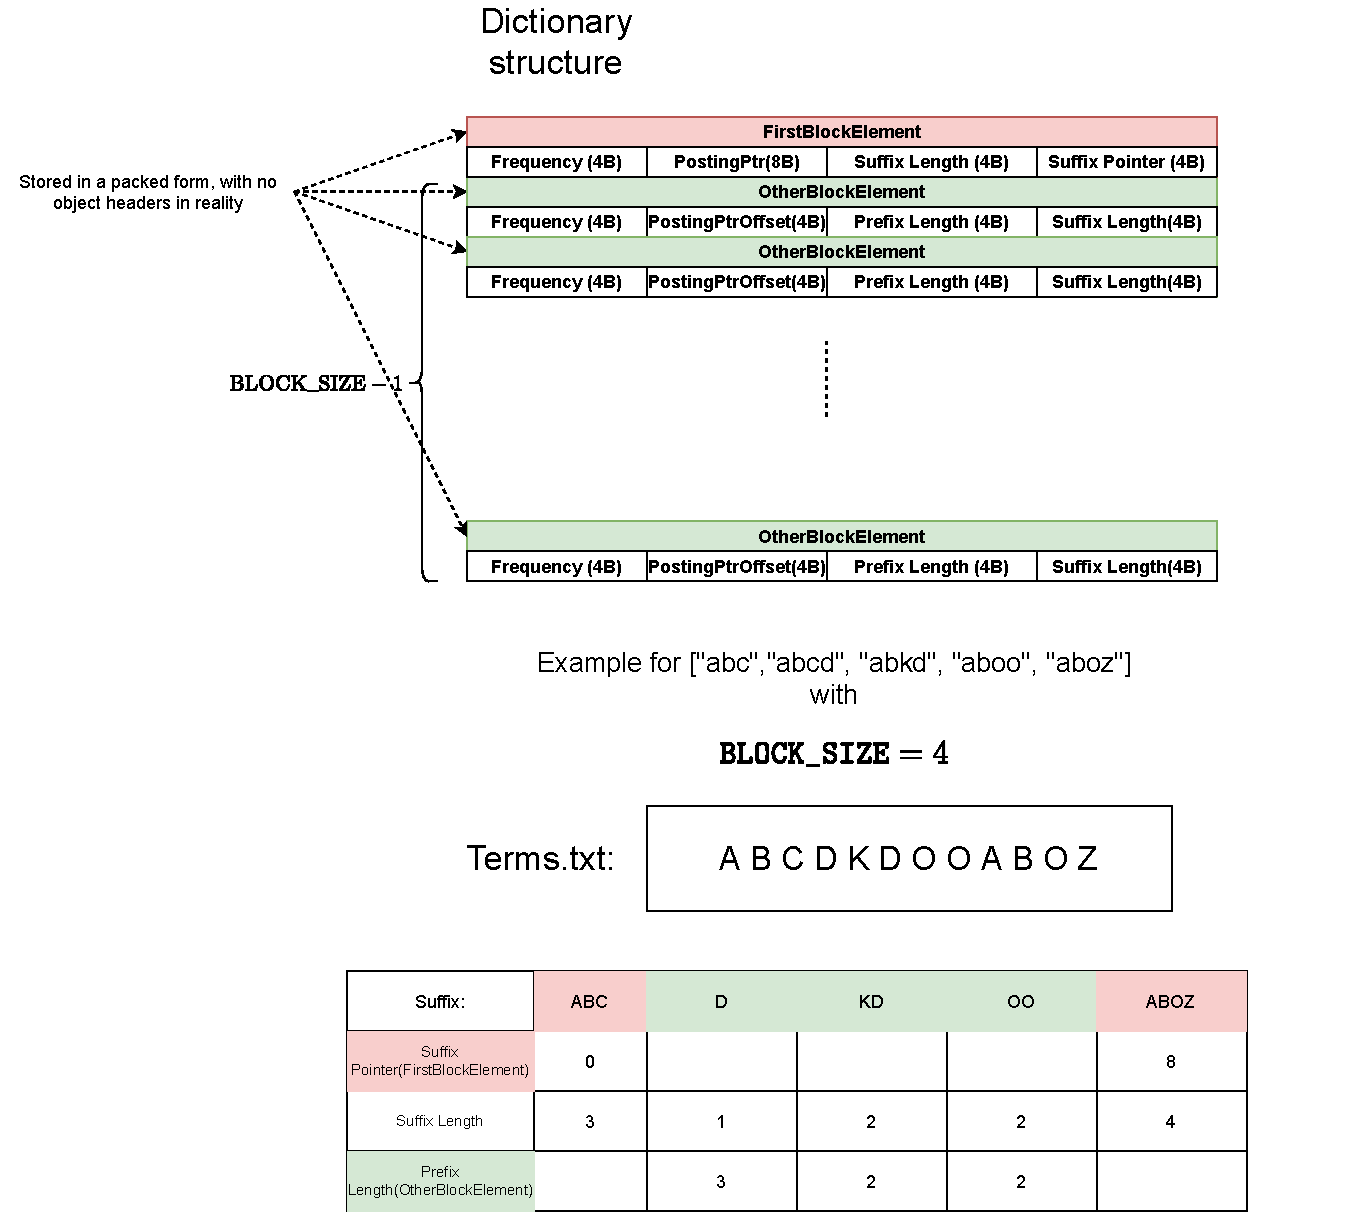
\includepdf[pages=-]{webdata_dictionary.pdf}
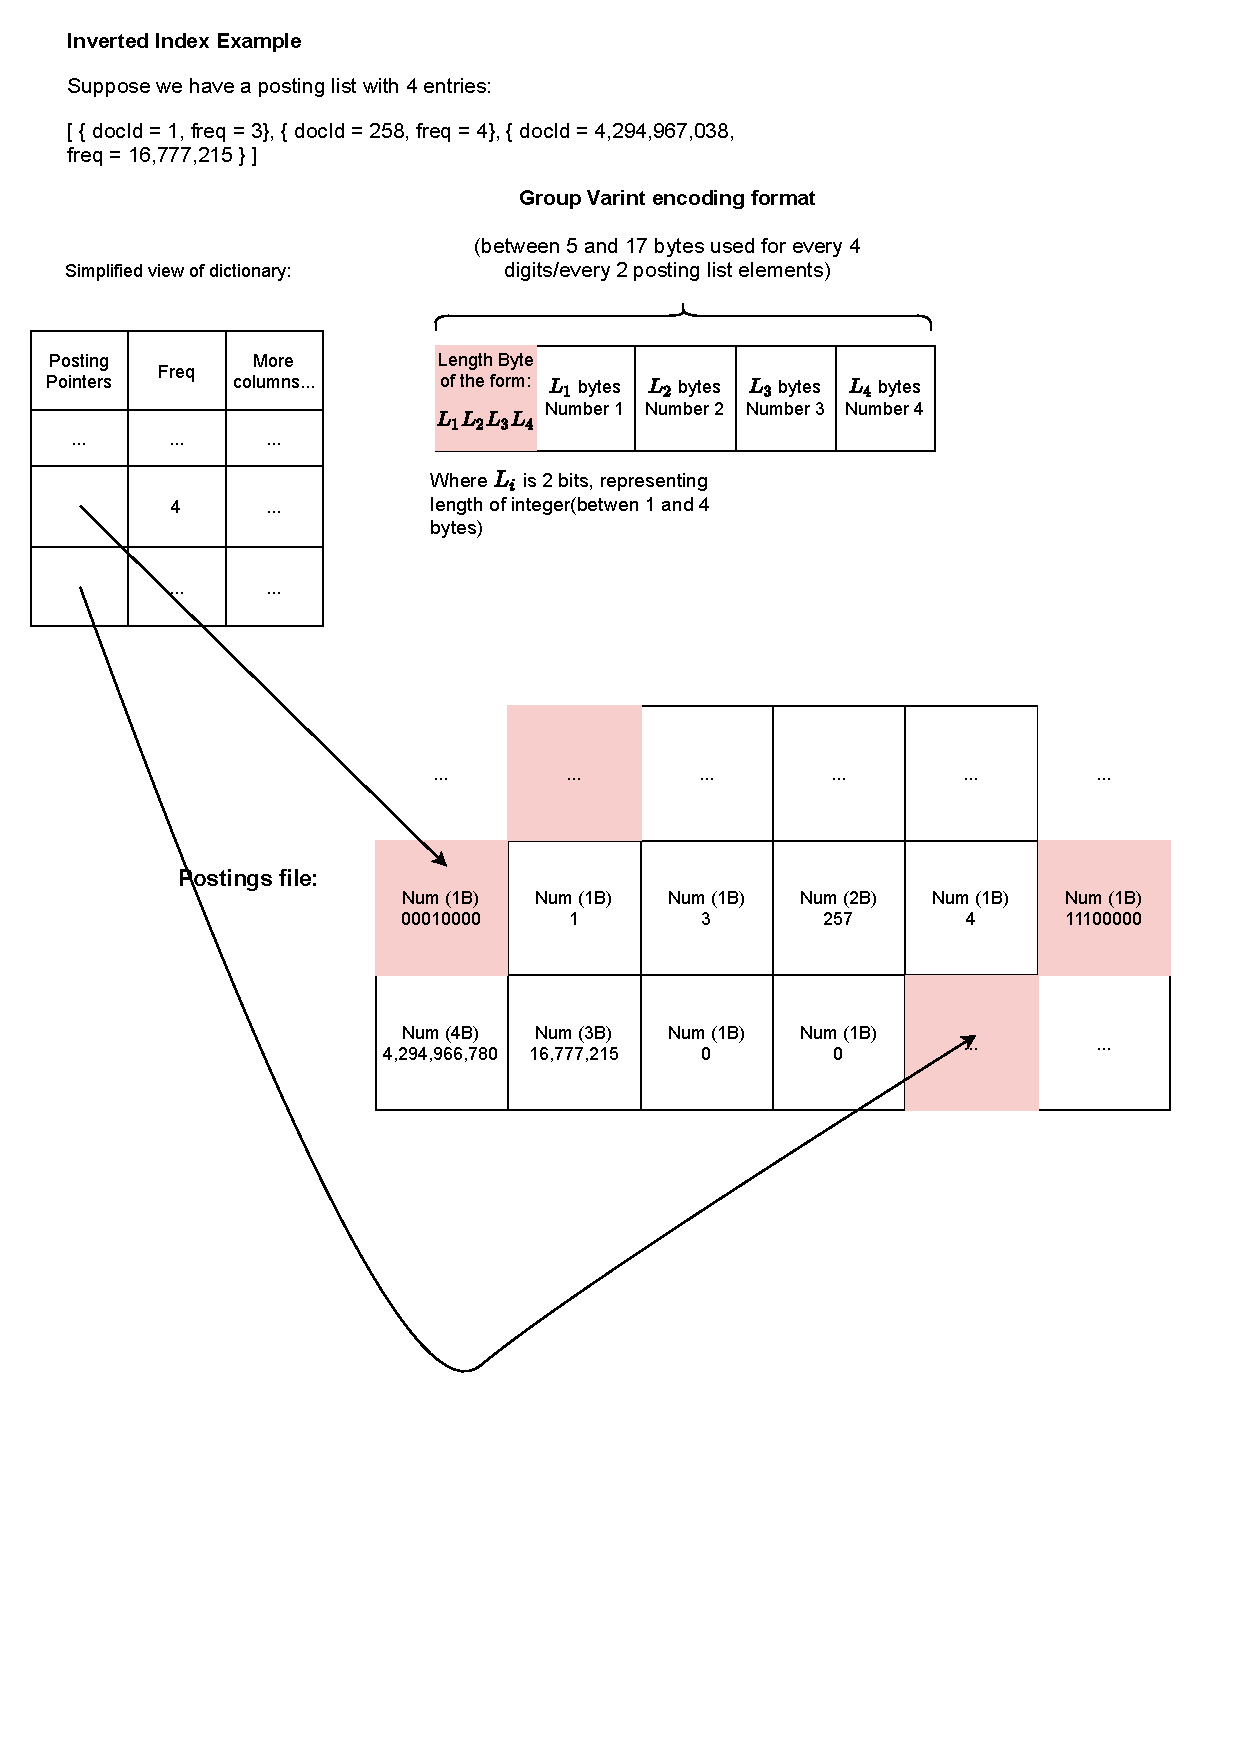
\includepdf[pages=-]{posting_list.pdf}
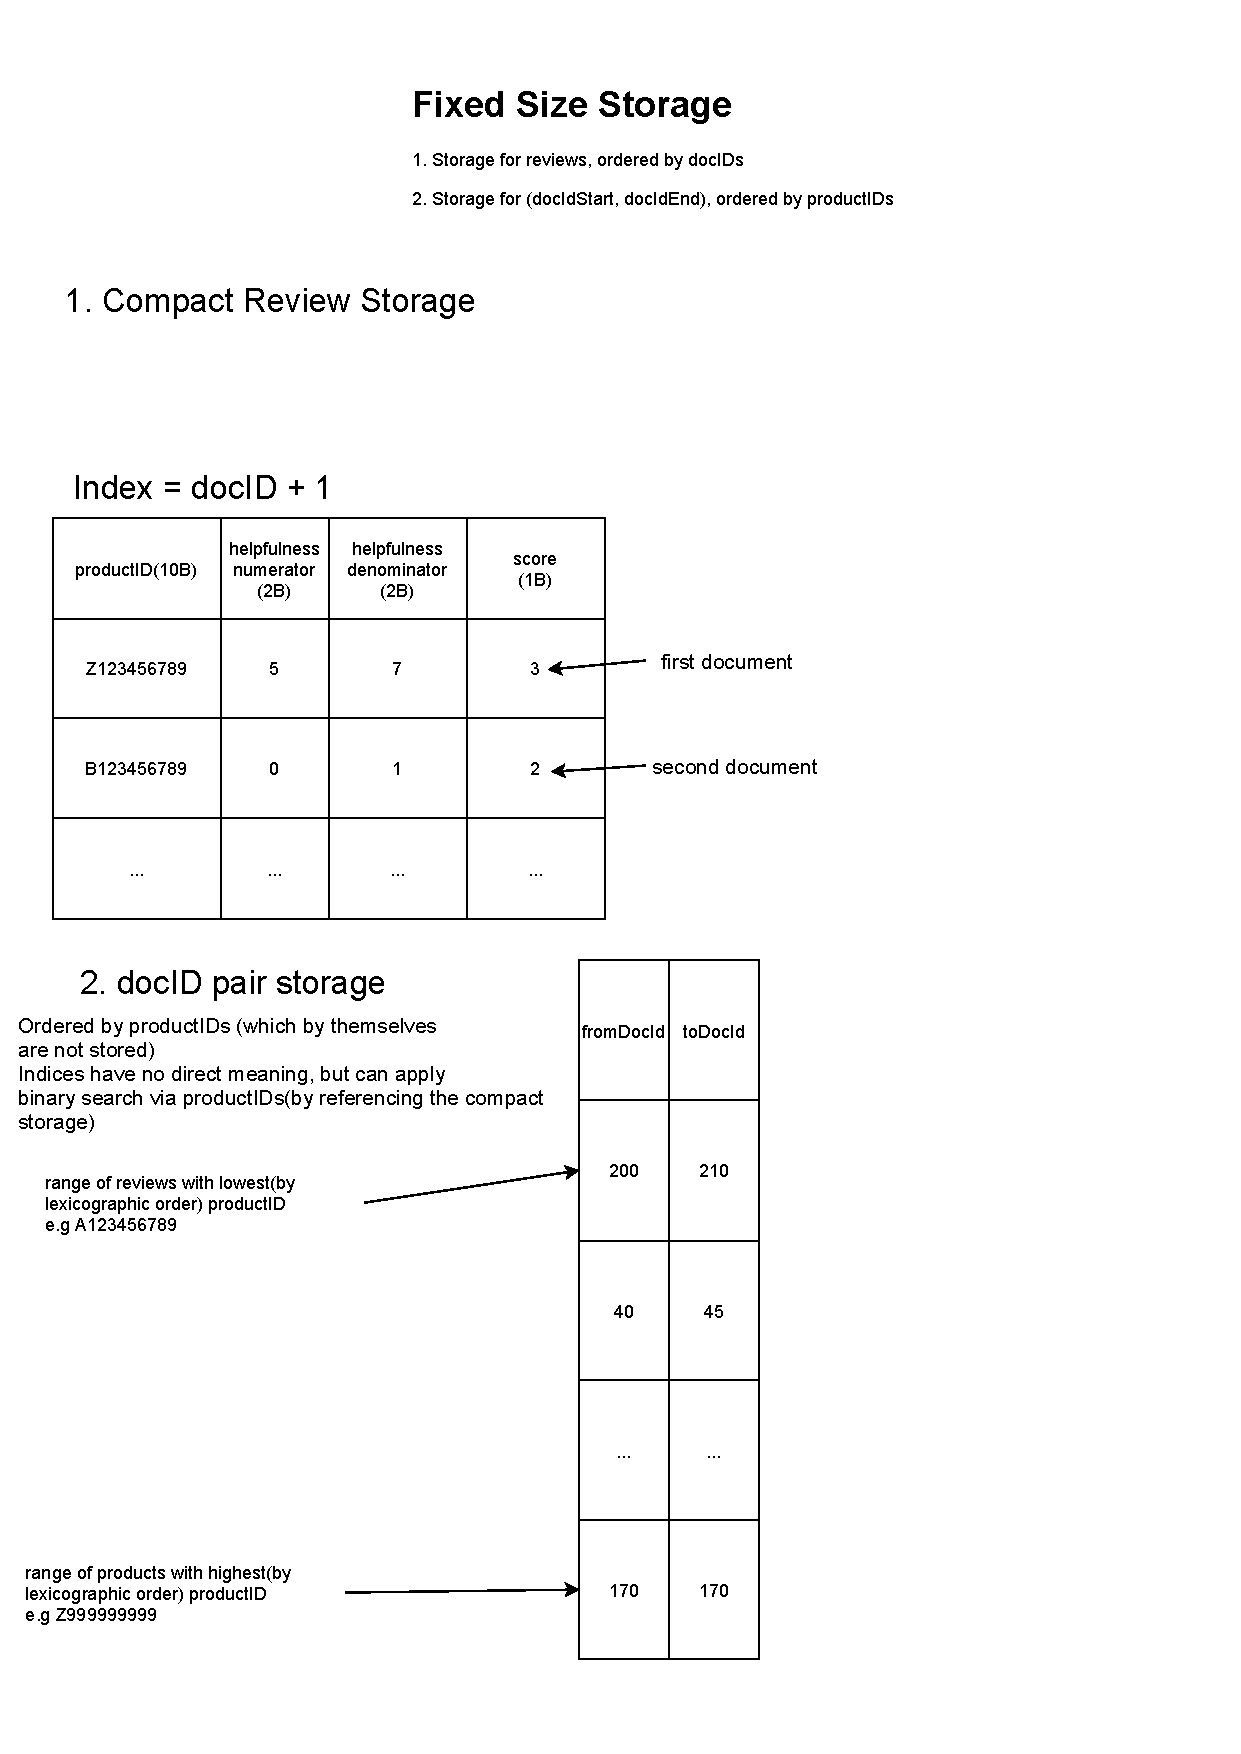
\includepdf[pages=-]{storage.pdf}

\subsection{Dictionary}

The dictionary uses (k-1)-in-k front-coding for compression, containing blocks of constant size, each block containing \verb+BLOCK SIZE+ terms
encoded via front-coding.

Each element in the block contains the token document frequency(length of posting list) and a posting pointer, in addition, the first block element
contains a suffix pointer and suffix length (allowing de-referencing its term), and every other block element contains a prefix length and suffix length. \footnote{In class we store the entire token's length rather than the suffix length. Overall this doesn't matter because 
	$\text{length} = \text{suffixLength} + \text{prefixLength}$}

Since other block elements do not include a suffix pointer, we need to de-reference every previous term in a block in order to determine the suffix
pointer. (Formally, $\texttt{suffixPointer}_i = \texttt{suffixPointer}_{i-1} + \texttt{suffixLength}_{i-1}$)

This implies a space-time trade-off with regards to block size, a higher block size allows better compression of the terms, but higher dictionary
search time.


There are a couple of optimizations that \textbf{I did not yet implement} due to time constraints:

\begin{itemize}

\item Shrinking suffix and prefix lengths, perhaps instead of using 4 bytes, 2 bytes or even 1 byte would suffice. I hypothesize that in a 
  large data-set these would be smaller, but this depends on the token distribution, average token length and other statistics..
  
  (I might implement this in the next exercise if I find this to be necessary)
  
\item Omitting the suffix length of the last block element, as it can probably be derived using the suffix pointer of the first element in the next block.
  
  Not implemented because the saving's don't seem particularly worthwhile and it just complicates the code
  
\end{itemize}


One important optimization that I did implement, is the use of a "packed" array (see class \verb+PackedDictionaryElements+), instead of
storing these blocks as plain Java objects, they are stored as bytes. This saves a lot of memory that would otherwise be wasted on object headers, at
cost of higher running time when reading those bytes as objects when trying to retrieve an element from the dictionary.

Another optimization is that the tokens(suffixes) aren't encoded in Java's UTF-16, rather, they use UTF-8, which should halve the memory
usage for data-sets which mostly use the Latin alphabet. This of course comes at a running-time cost when decoding the terms and translating them back into \verb+String+.

In addition, two integers, total number of reviews and token collection frequency, which were calculated during parsing, are stored in a separate file,
allowing $O(1)$ access.

\subsection{Inverted Index}

The inverted index consists of $D$ posting lists, each identified by a posting list pointer
and token document frequency(the length of the posting list)

Each posting list is a sequence of the form $(\texttt{docIdGap}_i, \texttt{frequency}_i)_i$ which are compressed using group varint encoding.


\subsection{Compact Review Storage}
\label{sec:compactStorage}

A "compact review" consists of the following fields:

\begin{itemize}
	\item Product ID (10 bytes)
	\item Score (1 byte)
	\item Helpfulness Numerator(2 bytes)
	\item Helpfulness Denominator(2 bytes)
	\item Number of tokens (4 bytes)
\end{itemize}

The compact review store is a file containing these records, ordered by review IDs. Since
each such review is of fixed size, it is possible to do $O(1)$ random access on the file
to obtain a review with a given review ID. 

\subsection{Product ID to docID Pair Storage}
\label{sec:pairStorage}

In order to allow $O(\log D)$ implementation of \verb+getProductReviews(String productId)+, 
there is a file containing $D$ fixed size records of the form $(fromDocId, toDocId, productID)$ ordered
by the product IDs. Each record represents the range of reviews
for said product.

The fact the product ID stored on both the compact review storage as well as the pair storage might seem wasteful, but it reduces time spent on IO
while doing binary search and allows better utilization of cache locality.


\section{Main Memory Versus Disk}

\begin{comment}
{\em Put an explanation of which portions of the index are read into memory when an IndexReader object is created, and which portions will be read as needed. }
\end{comment}

The token strings are loaded into memory, as well as the elements of the dictionary (in a packed form), and some statistics (token collection frequency
and number of reviews)

The "compact reviews", "product ID to docID pairs" and posting lists are kept on disk. I use Java's buffered reader class when reading postings, which
might load a few more kilobytes into memory, but they essentially take constant memory.

\section{Theoretical Analysis of Size}

\begin{comment}
{\em Theoretically analyze the expected size (in bytes) of all of your index structures. In your
  analysis, the size of the index should be a function of the size of the
  input.  Use the following variables to denote the various input size parameters:
}
\end{comment}
  \begin{description}
      \item[$N$] Number of reviews
      \item[$M$] Total number of tokens (counting duplicates as many times as they appear)
      \item[$D$] Number of different tokens (counting duplicates once)
      \item[$L$] Average token length (counting each token once)
      \item[$F$] Average token frequency, i.e., number of reviews containing a token
      \item[$P$] Number of different products (namely $P = O(N)$)
      \item[$R$] Average number of different reviews in which a token appears. (Namely, $R = O(N)$)
  \end{description}


\begin{description}	
	\item[Dictionary] $O(D \cdot L))$ 
	
	If we ignore front-coding or if all tokens don't share any suffixes, then the average space taken by
	the strings is $O(D \cdot L)$. Since $\texttt{BLOCK\_SIZE} \ll D$ then it's clear that even with front-coding,
	there's no asymptotic difference in the file size with (k-1)-in-k front coding in contrast to plain string concatenation.
	
	As for the contents of the dictionary itself, we have $D$ elements and each dictionary element takes a fixed amount of bytes,
	thus the dictionary contributes $O(D)$ memory, so in total we have a space complexity of $O(D \cdot L)$
	

	\item[Inverted Index] $O(\frac{M}{F})$
	
	On average, every $F$ occurrences of some token will belong to the same document, thus
	they will be encoded as a single tuple within some posting list, giving us a total of
	 $O(\frac{M}{F})$ tuples in the posting list.
	 
	 Each tuple is of constant size, containing the docID gap and the document frequency,
	 each using between 1 and 4 bytes(encoded via group-varint encoding), giving us a space complexity of $O(\frac{M}{F})$
	 
	 
	\item[Compact Review Storage] $\O(N)$
	 
	Mostly explained in \hyperref[sec:compactStorage]{a previous section} - we have $N$ records of fixed size
	 
	\item[Product ID to docID Pair Storage] $O(P)$ 
	 
	 Mostly explained in \hyperref[sec:pairStorage]{a previous section} - we have $P$ records and each only uses 2 integers and 10 bytes(18 bytes per record)
	 
\end{description}
  
\section{Theoretical Analysis of Runtime}  

\begin{comment}
{\em Using the same variables, theoretically analyze the runtime of the functions of IndexReader. Include both the runtime and a short explanation.}
\end{comment}

\begin{itemize}
    \item \verb+IndexReader(String dir)+: $O(D\cdot L)$
    
    The token strings(without repetitions of course) are held within memory
    The dictionary is loaded into memory:
    
    The token strings are held in a memory mapped file, which ideally(enough RAM) would be loaded in its entirety to disk, using $O(D\cdot L)$ space.
    The dictionary structure(essentially an array of fixed size records between 3
    and 4 ints) is itself $O(D)$, therefore the total running time is $O(D\cdot L)$

    \item \verb+getProductId(int reviewId)+: $O(1)$
    
    See \hyperref[sec:compactStorage] {compact storage}, can access a review entry via random access based on docID.

	\item \verb+getReviewScore(int reviewId)+: $O(1)$
	
	See \hyperref[sec:compactStorage] {compact storage}, can access a review entry via random access based on docID.	

	\item \verb+getReviewHelpfulnessNumerator(int reviewId)+: $O(1)$
    
    See \hyperref[sec:compactStorage] {compact storage}, can access a review entry via random access based on docID.

   \item \verb+getReviewHelpfulnessDenominator(int reviewId)+: $O(1)$

    See \hyperref[sec:compactStorage] {compact storage}, can access a review entry via random access based on docID.

   \item \verb+getReviewLength(int reviewId)+: $O(1)$

    See \hyperref[sec:compactStorage] {compact storage}, can access a review entry via random access based on docID.
    (The review length is computed when creating the compact storage during parse-time, by \verb+SlowIndexWriter+)

	\item \verb+getTokenFrequency(String token)+: $O(\log D)$
	
	Binary search in the dictionary takes $O(\log D)$, the token frequency is stored in the dictionary
	element so can be obtained in $O(1)$ once we found the position within the dictionary.
    
    \item \verb+getTokenCollectionFrequency(String token)+: $O(\log(D) + R)$

	First, finding the posting list(and its length/token's length) takes $O(\log D)$
	
	As I defined before, the average token appears in $O(R)$ different reviews, which is
	the size of its posting list/document frequency, giving us a cost of $O(R)$ to
	iterate the posting list and sum up the frequencies to obtain the collection frequency.
	
    \item \verb+getReviewsWithToken(String token)+: $O(\log D)$ if we don't iterate over the enumeration, otherwise $O(\log(D) + R)$
    
    Producing the enumeration(an iterator) only requires finding the posting pointer and document frequency of a given token, which like I explained above,
    is $O(\log D)$. Iterating over the entire enumeration would take $O(R)$ as we'd iterate over the posting list.

    \item \verb+getNumberOfReviews()+: $O(1)$
    
    Stored in the \verb+Dictionary\verb+ object as a custom field, was calculated by \verb+SlowIndexWriter+ when parsing the input file.

    \item \verb+getTokenSizeOfReviews()+: $O(1)$
    
    Same as above

   \item \verb+getProductReviews(String productId)+: $O(\log P)$ if we don't iterate over the enumeration, otherwise $O(\log P + \frac{N}{P}))$
   
 
   To build the enumeration we simply need the lowest and highest docIDs of reviews for a product, which are stored in a single element within the docID
   pair storage, which is ordered by product IDs(see \hyperref[sec:pairStorage]{before}), thus we can perform binary search over said file in $O(\log P)$
   
   If we include the iteration of the enumeration - splitting the $N$ reviews over $P$ sets of products(on average), means the average product has
   $\frac{N}{P}$ reviews, which is the size of the enumeration.

\end{itemize}

\end{document}
